\section{\label{sec:kbpo:kbpo} Implementing on-demand evaluation as an online service}



We implemented the on-demand evaluation framework described here as a publicly available evaluation service dubbed KBP Online\footnote{Accessible at \url{https://kbpo.stanford.edu}}.
We integrated the crowdsourcing interfaces described in \refsec{application} to dynamically launch crowdsourcing tasks as 

asynchronous turking requests

Implementing query distributions

\begin{figure}
  \centering
  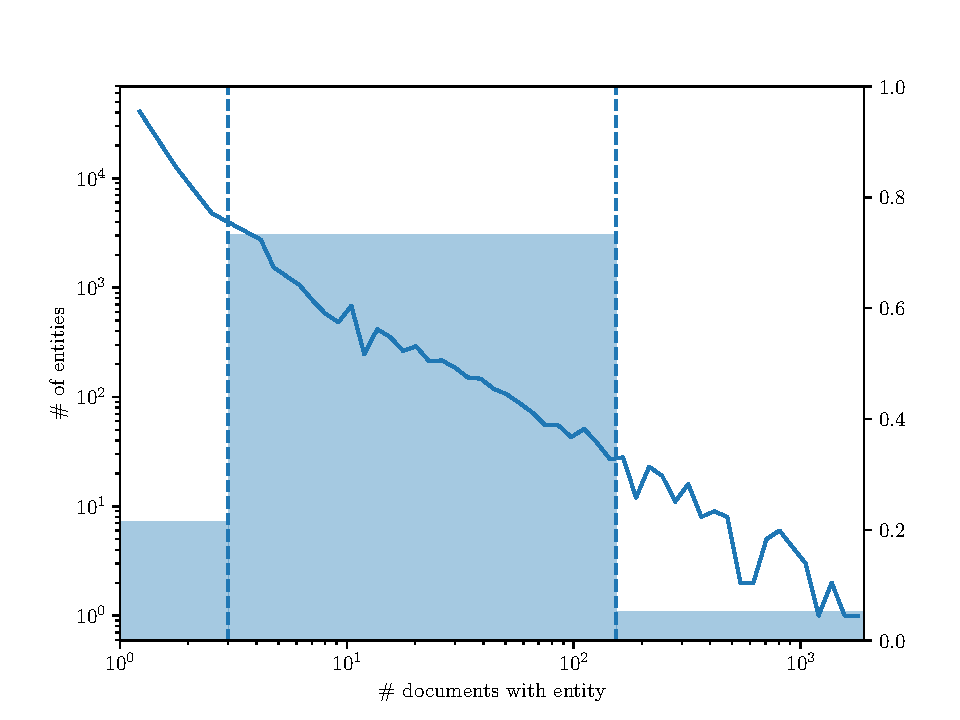
\includegraphics[width=0.8\textwidth]{figures/analysis/distribution}
  \caption[TAC KBP 2016 Query entity distribution]{\label{fig:kbpo:distribution}
    The solid line plots a histogram of how many documents a particular entity appeared in the TAC KBP 2016 corpus.
    The distribution is approximately a power-law distribution.
    Overlayed is a histogram of the frequency of the actual query entities used in the TAC KBP 2016 evaluation, binned by their frequency. We consider entities that appear in 3 or less unique documents (the 50th percentile) to be ``low'' frequency entities, those that appear more than 154 unique document (90th percentile) to be ``high'' frequency entities and those that appear in between to be ``medium'' frequency entities.
    The TAC KBP 2016 evaluation has a clear preference for medium frequency followed by low frequency entities.
  }
\end{figure}

\begin{figure}
  \centering
  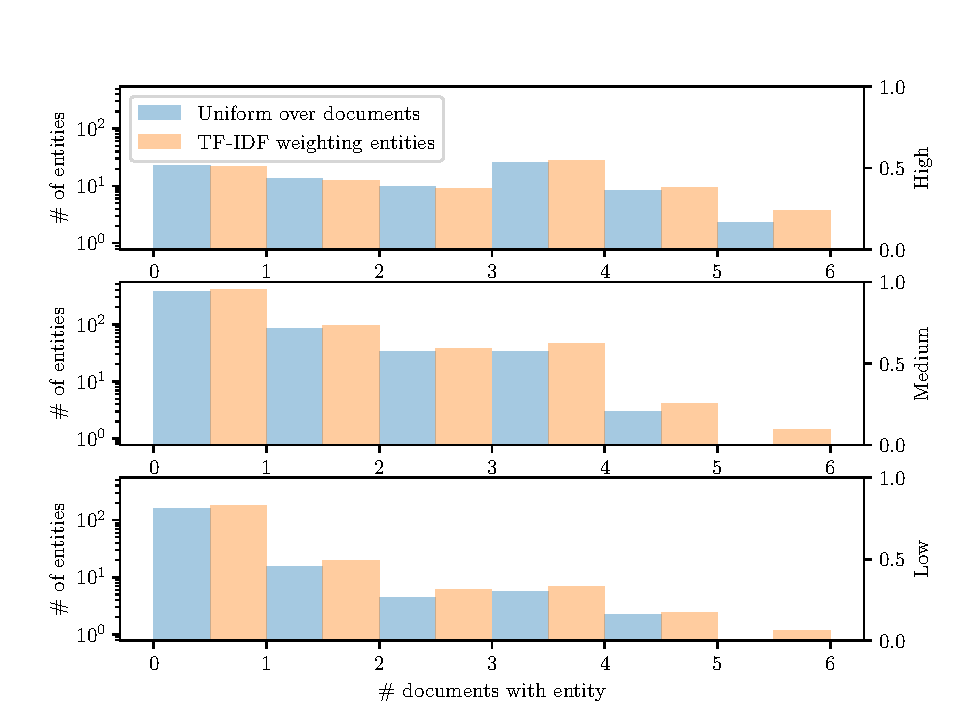
\includegraphics[width=0.8\textwidth]{figures/analysis/exhaustive_entity_cross}
  \caption[Comparison of document sampling distributions]{\label{fig:kbpo:exhaustive_entity_cross}
  In order to properly test the entity linker when measuring recall, an important feature of KBP systems, we must identify documents for exhaustive annotation that contain some entity clusters.
  A sample of 200 documents uniformly picked from the document collection only exhibits clusters for high frequency entities.
  Our TF-IDF sampling scheme is able to ensure that even medium and low frequency entities appear across multiple documents in the sample.
  }
\end{figure}

\begin{figure}
  \centering
  \begin{subfigure}{0.8\textwidth}
    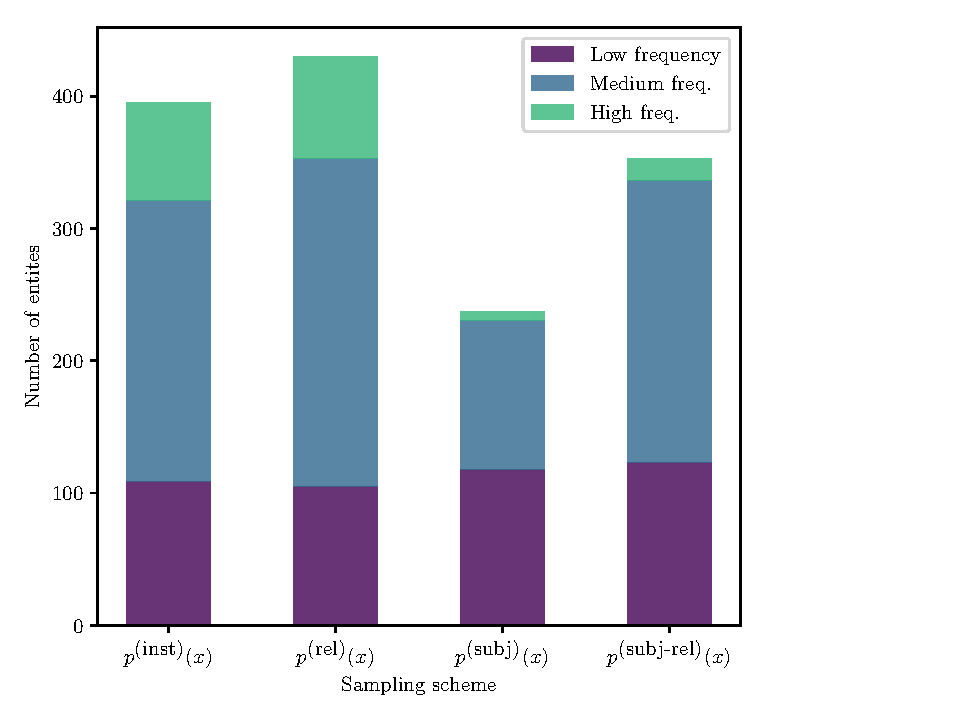
\includegraphics[width=\textwidth]{figures/analysis/selective_supervised_entity}
    \caption{Entity distribution}
  \end{subfigure}

  \begin{subfigure}{0.8\textwidth}
    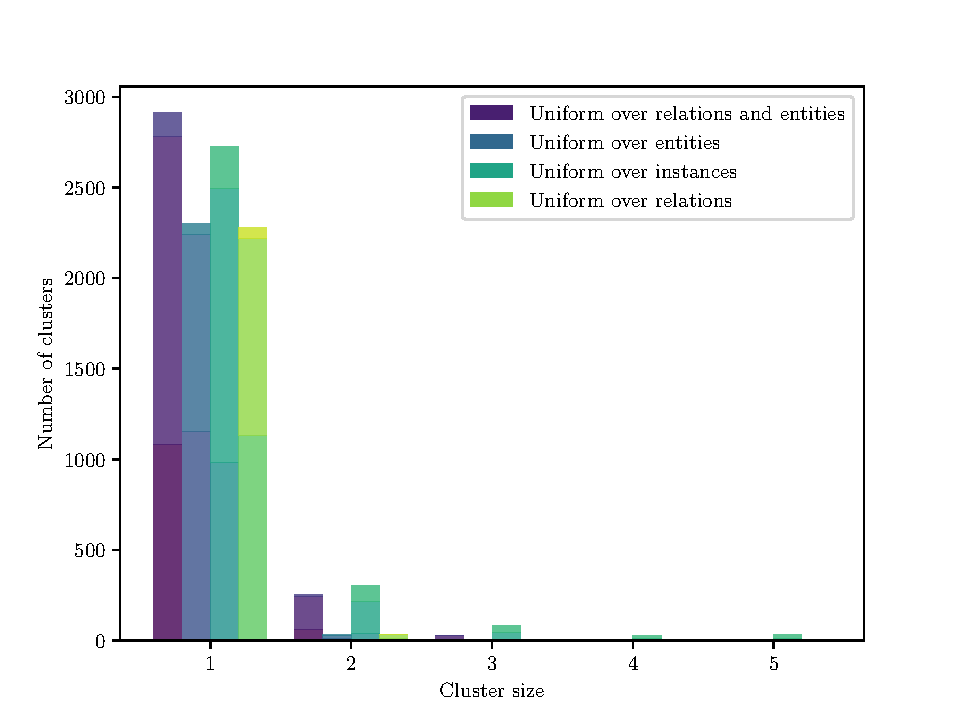
\includegraphics[width=\textwidth]{figures/analysis/selective_supervised_clusters}
    \caption{Entity cluster distribution}
  \end{subfigure}

  \caption[Comparison of relation sampling distributions]{\label{fig:kbpo:selective_supervised_entity}
  }
\end{figure}

\begin{figure}
  \centering
  \begin{subfigure}{\textwidth}
    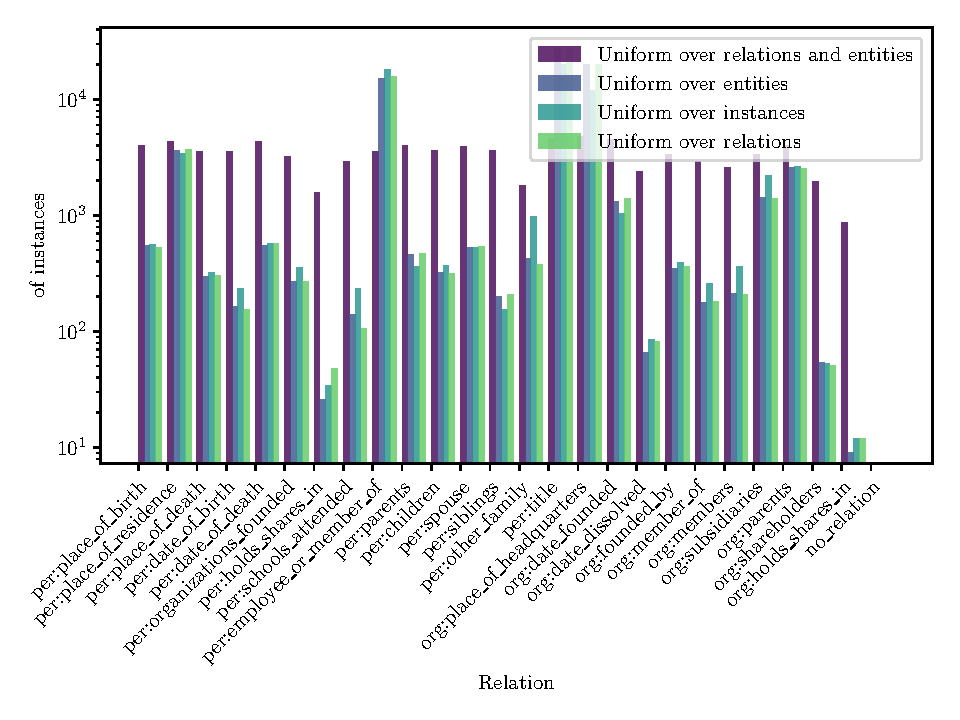
\includegraphics[width=\textwidth]{figures/analysis/selective_supervised_relations}
    \caption{Relation distribution}
  \end{subfigure}

  \caption[Comparison of relation sampling distributions]{\label{fig:kbpo:selective_supervised_relation}
  }
\end{figure}



\begin{figure}
  \centering
  \begin{subfigure}{0.8\textwidth}
    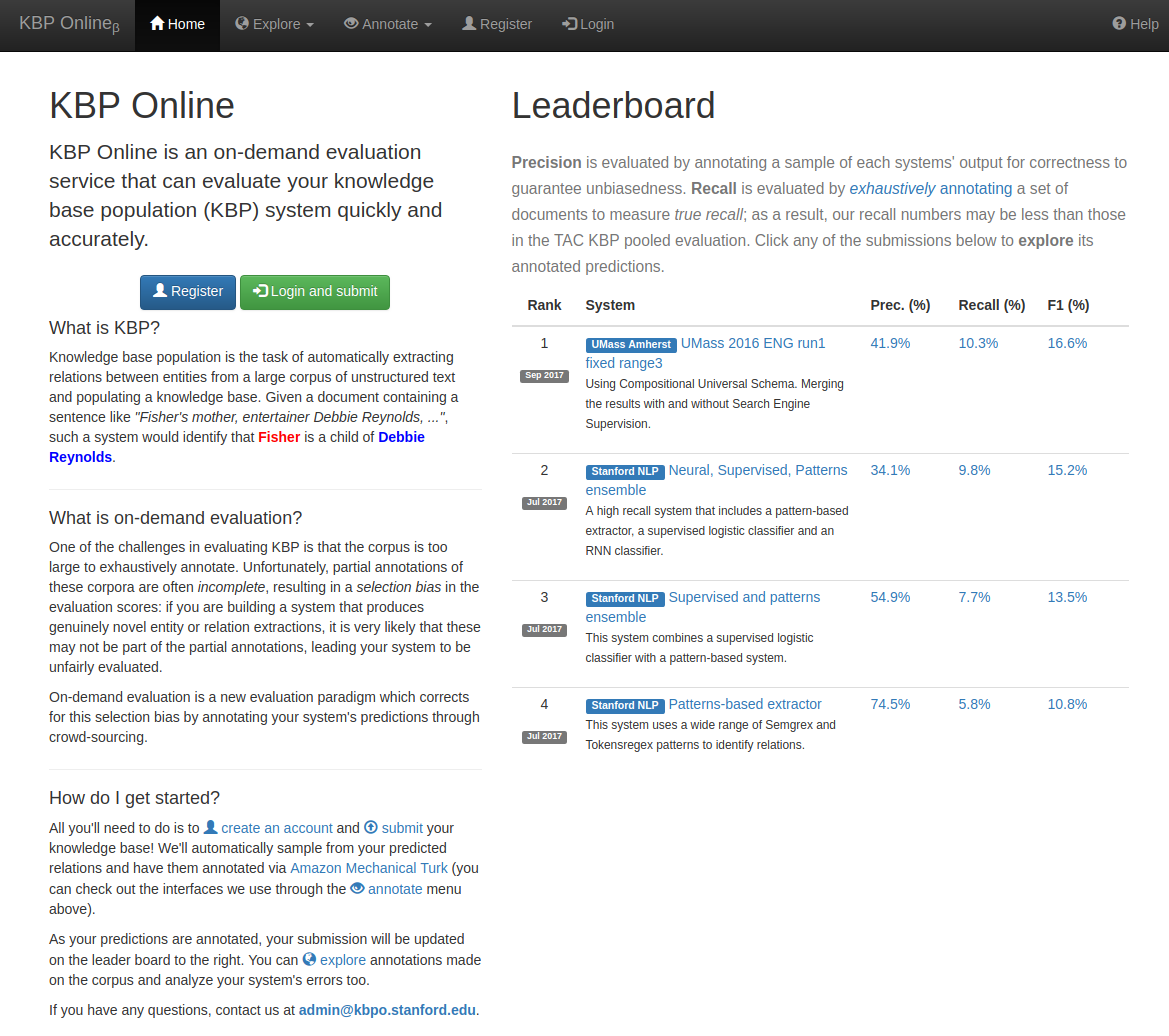
\includegraphics[width=\textwidth]{figures/interface/leaderboard}
    \caption{Leaderboard}
  \end{subfigure}

  \begin{subfigure}{0.8\textwidth}
    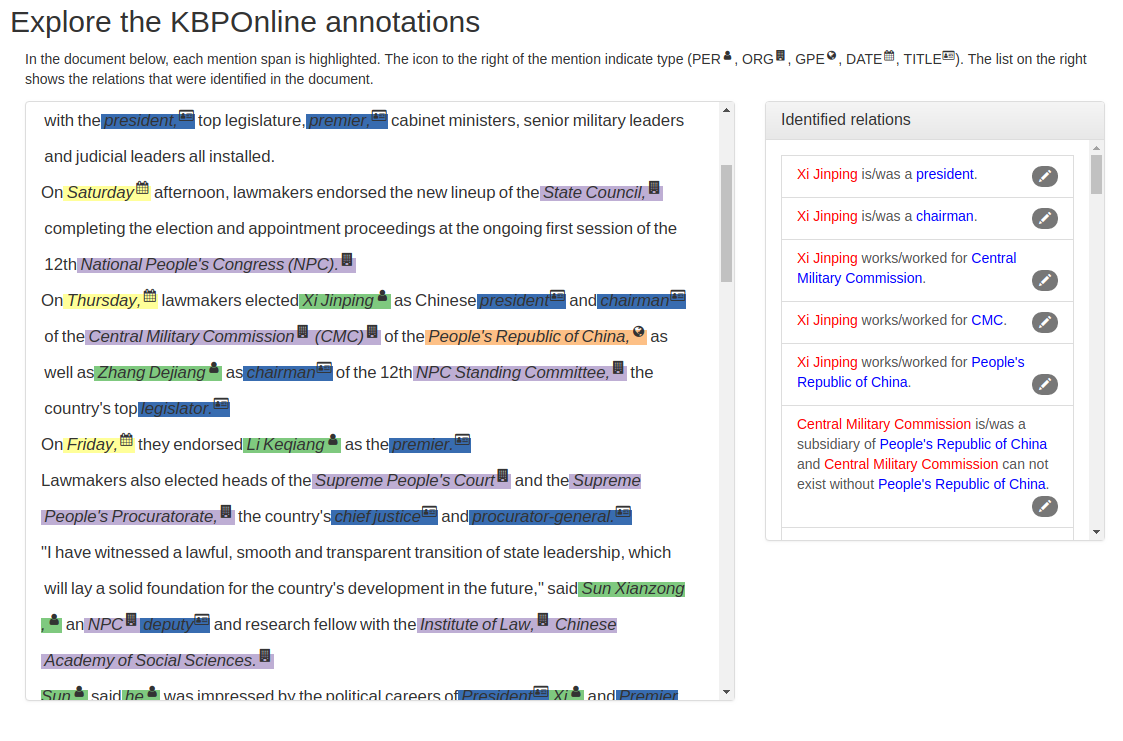
\includegraphics[width=\textwidth]{figures/interface/explore-data}
    \caption{Explore annotations}
  \end{subfigure}

  \begin{subfigure}{0.8\textwidth}
    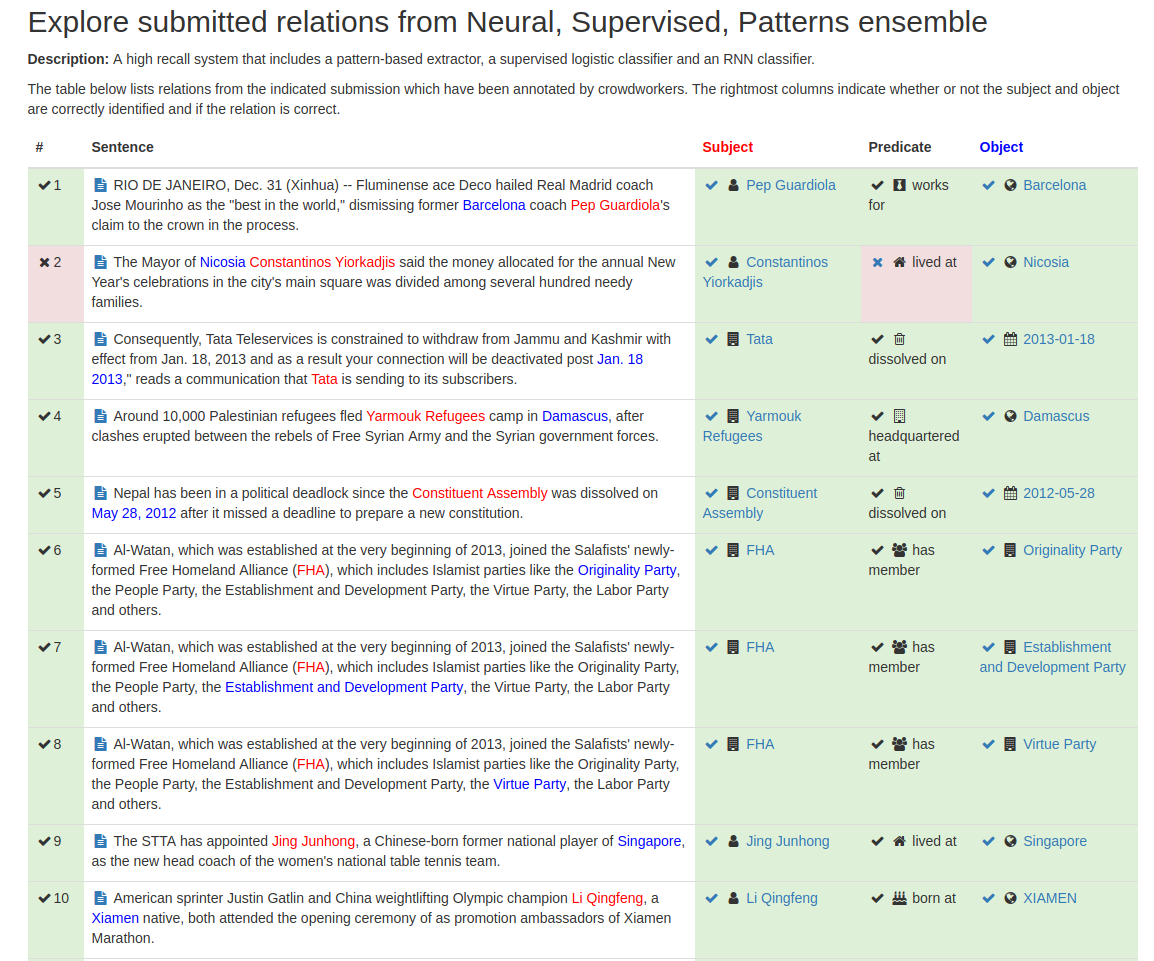
\includegraphics[width=\textwidth]{figures/interface/errors}
    \caption{Error analysis}
  \end{subfigure}

  \caption[Comparison of relation sampling distributions]{\label{fig:kbpo:selective_supervised_relation}
  }
\end{figure}



Exhaustive entity distribution for recall

Tradeoffs

Plot

sampling from the set of true documents.

Sampling from systems

Tradeoffs

Proposed sampling distribution.

Implementation details and challenges

* Handling entity linking
* Splitting scores into three components, based on error type

